\chapter{Planificación de caja}\label{chp-04}

\lettrine[lraise=-0.1, lines=2, loversize=0.2]{P}ara que todos los dispositivos que componen el sistema estén bien aislados del exterior
y no haya problemas con las conexiones se planifica una caja estanca. Ésta deberá ser 
accesible para el reemplazo de dispositivos defectuosos y ser replicable. 

Como referencia se toma de una caja de dimensiones 220 x 145 x 80 mm. Para reducir los 
costes, se decide imprimirla en 3D, ya que permite mayor adaptabilidad para colocar 
los lugares donde fijar los diferentes dispositivos. La caja estará dividida en una base y una 
tapa que se unen mediante tornillos y permiten una unión estable.

\section{Base}

La base debe tener las siguientes características:
\begin{itemize}
    \item Permitir fijar y extraer con facilidad todos los dispositivos. 
    \item Orificio para entrada de cables de conexión.
    \item Hueco para conector hembra Ethernet.
    \item Hueco para conector de pines digitales.
\end{itemize} 

Con todo ello se ha diseñado la base que se puede ver en la figura \ref{fig:cajabase}. Se muestra
una imagen de la planta y otra general. Se puede observar que cuenta con distintos orificios en los
que se debe introducir tuercas M3 durante la impresión en 3D para los distintos anclajes de dispositivos
que se comenta a continuación y para la unión con la tapa para que quede estanca la caja.

Además, para el anclaje de los dispositivos sobre la base, se ha diseñado un soporte que va atornillado
a la misma. Para ello, se ha modelado de forma simplificada todos los dispositivos y se ha buscado la 
forma óptima de disponerlos. También se ha tenido en cuenta los cables que van conectados tanto a la 
fuente como al Arduino, modelándolos en el espacio que ocupan hasta que el ángulo de giro es aceptable
para que el cable se pueda colocar de forma holgada y sin tensiones dentro de la caja.
Posteriormente se ha creado el soporte en base a dicha disposición y contando con los orificios de cada
dispositivo. En la figura \ref{fig:ensamblajebase} se puede observar el resultado final de este ensamblaje.

\newpage

\begin{figure}[htpb]% 
    \centering 
    \subfloat[][]{% 
        \label{fig:cajabasevista}% 
        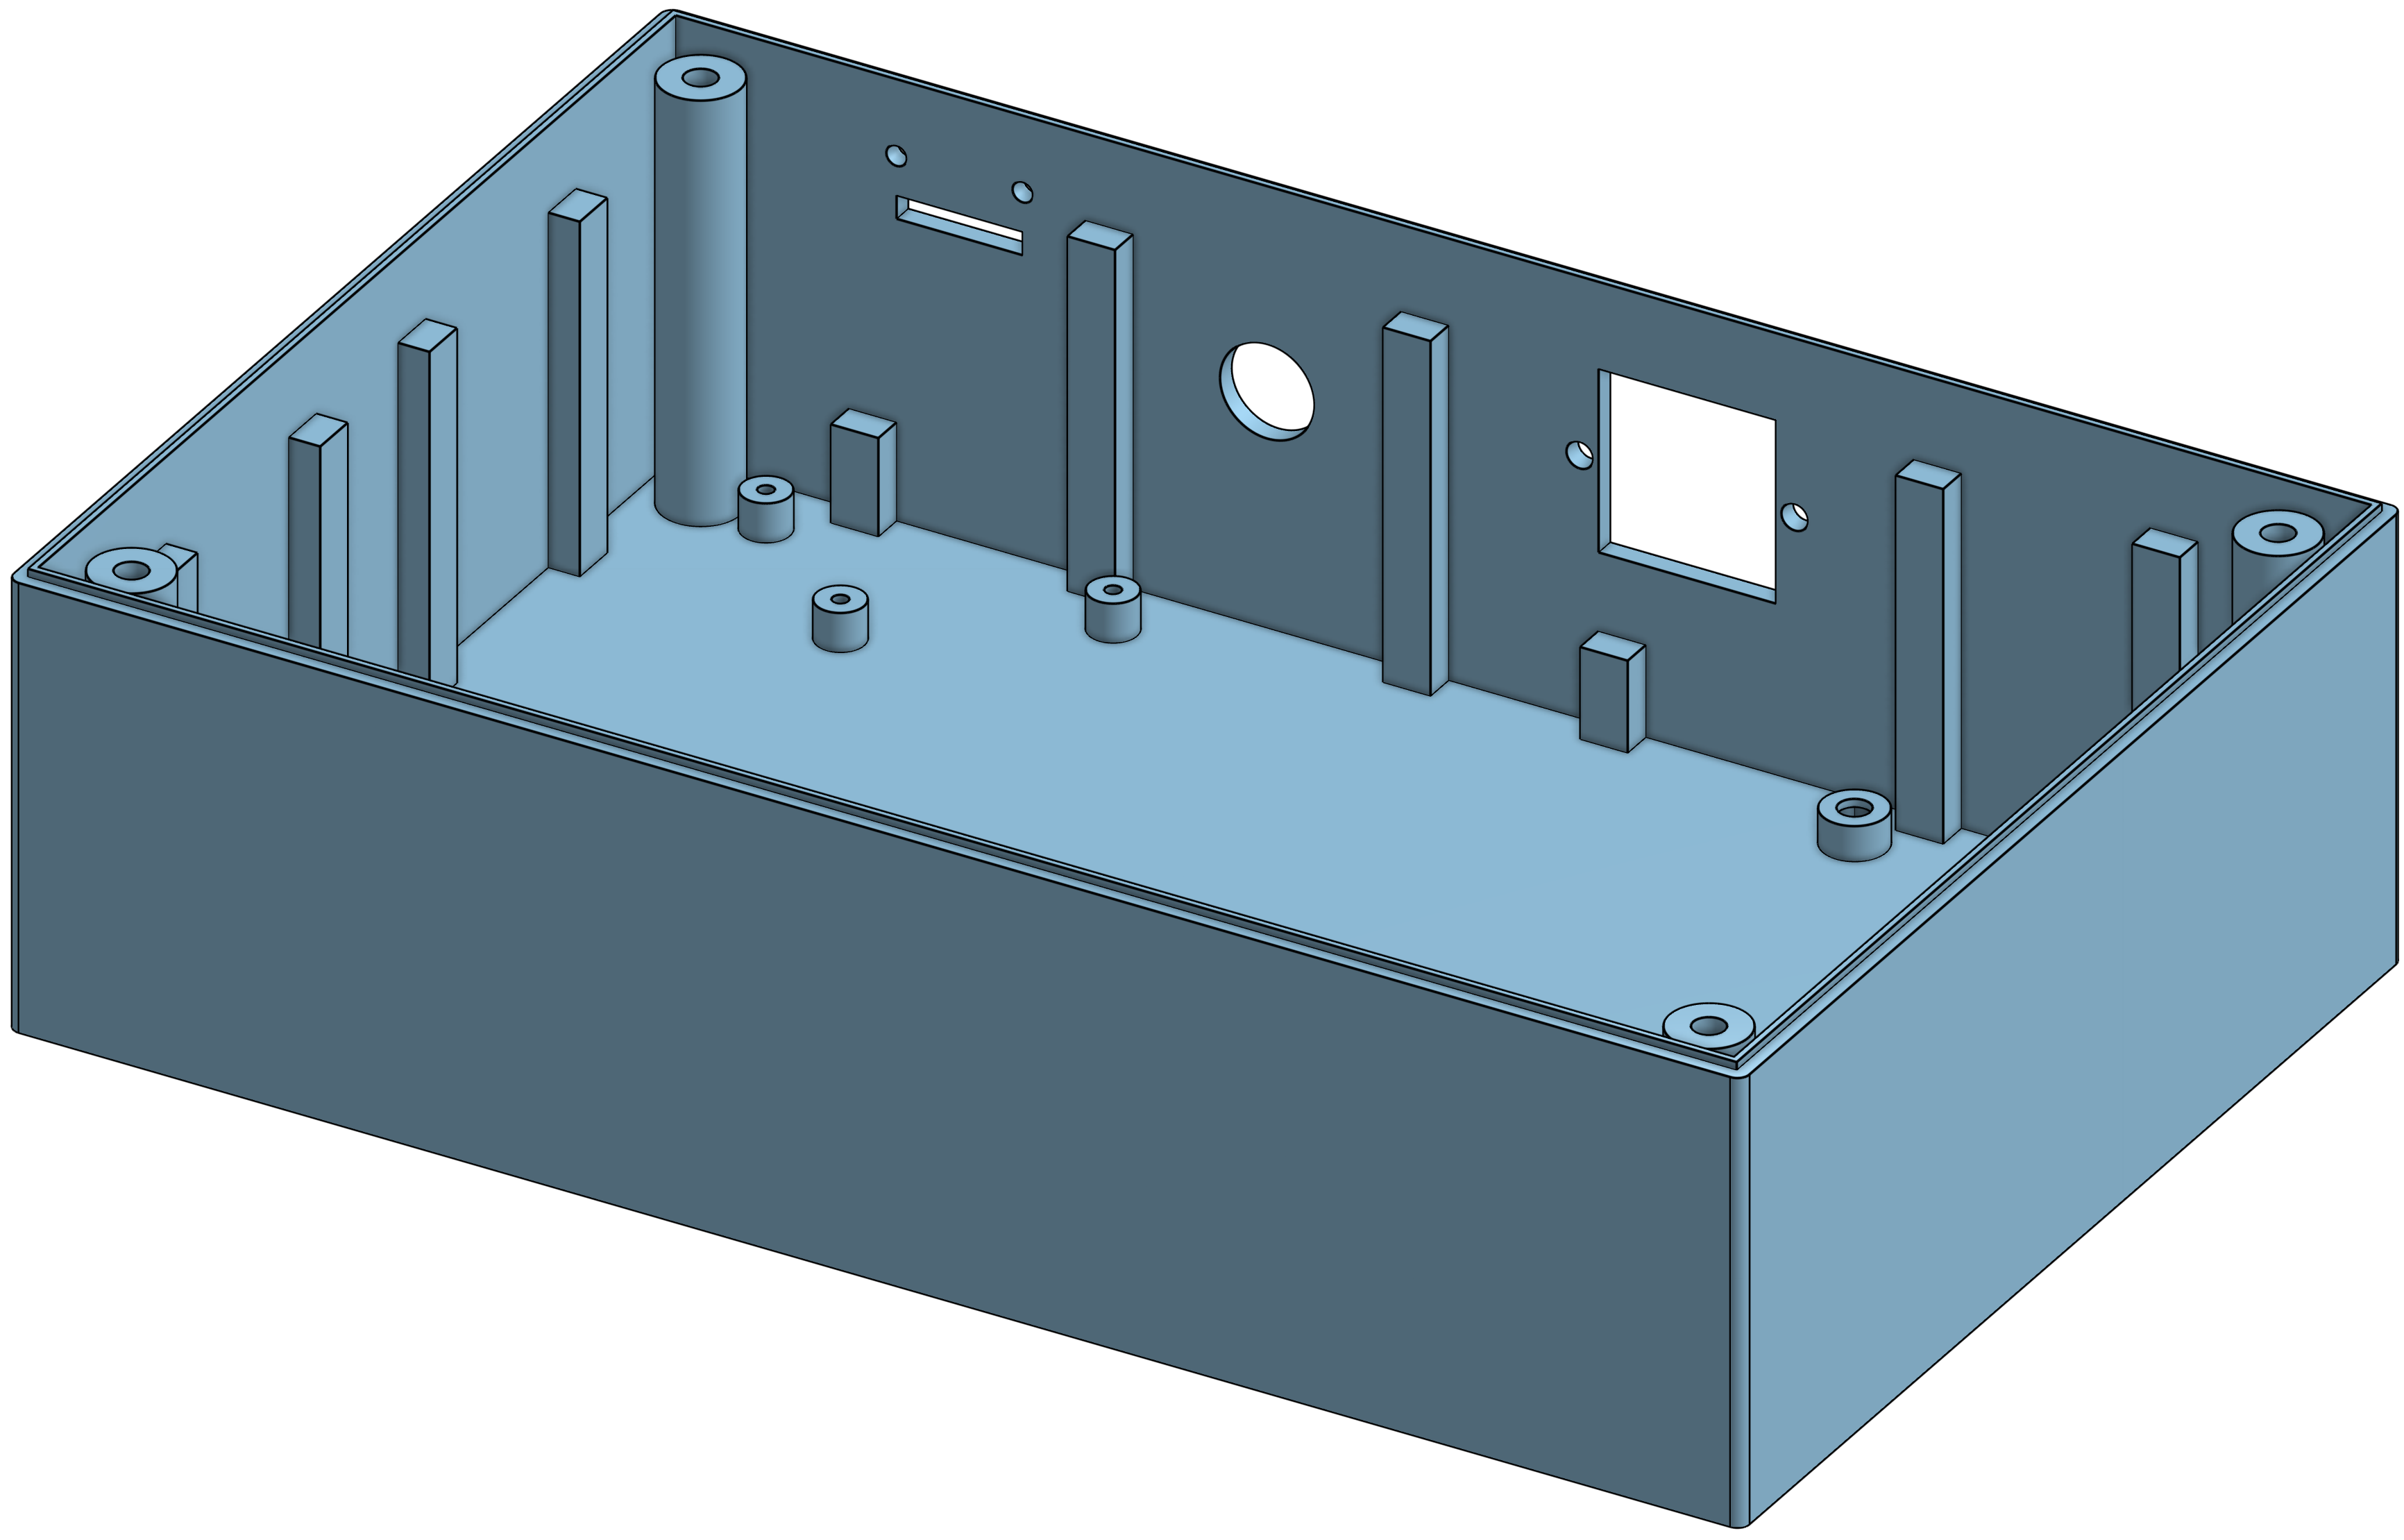
\includegraphics[width=0.5\textwidth]{04-caja/cajabase.png}
    }% 
    \hspace{10pt}% 
    \subfloat[][]{% 
        \label{fig:cajabaseplanta}% 
        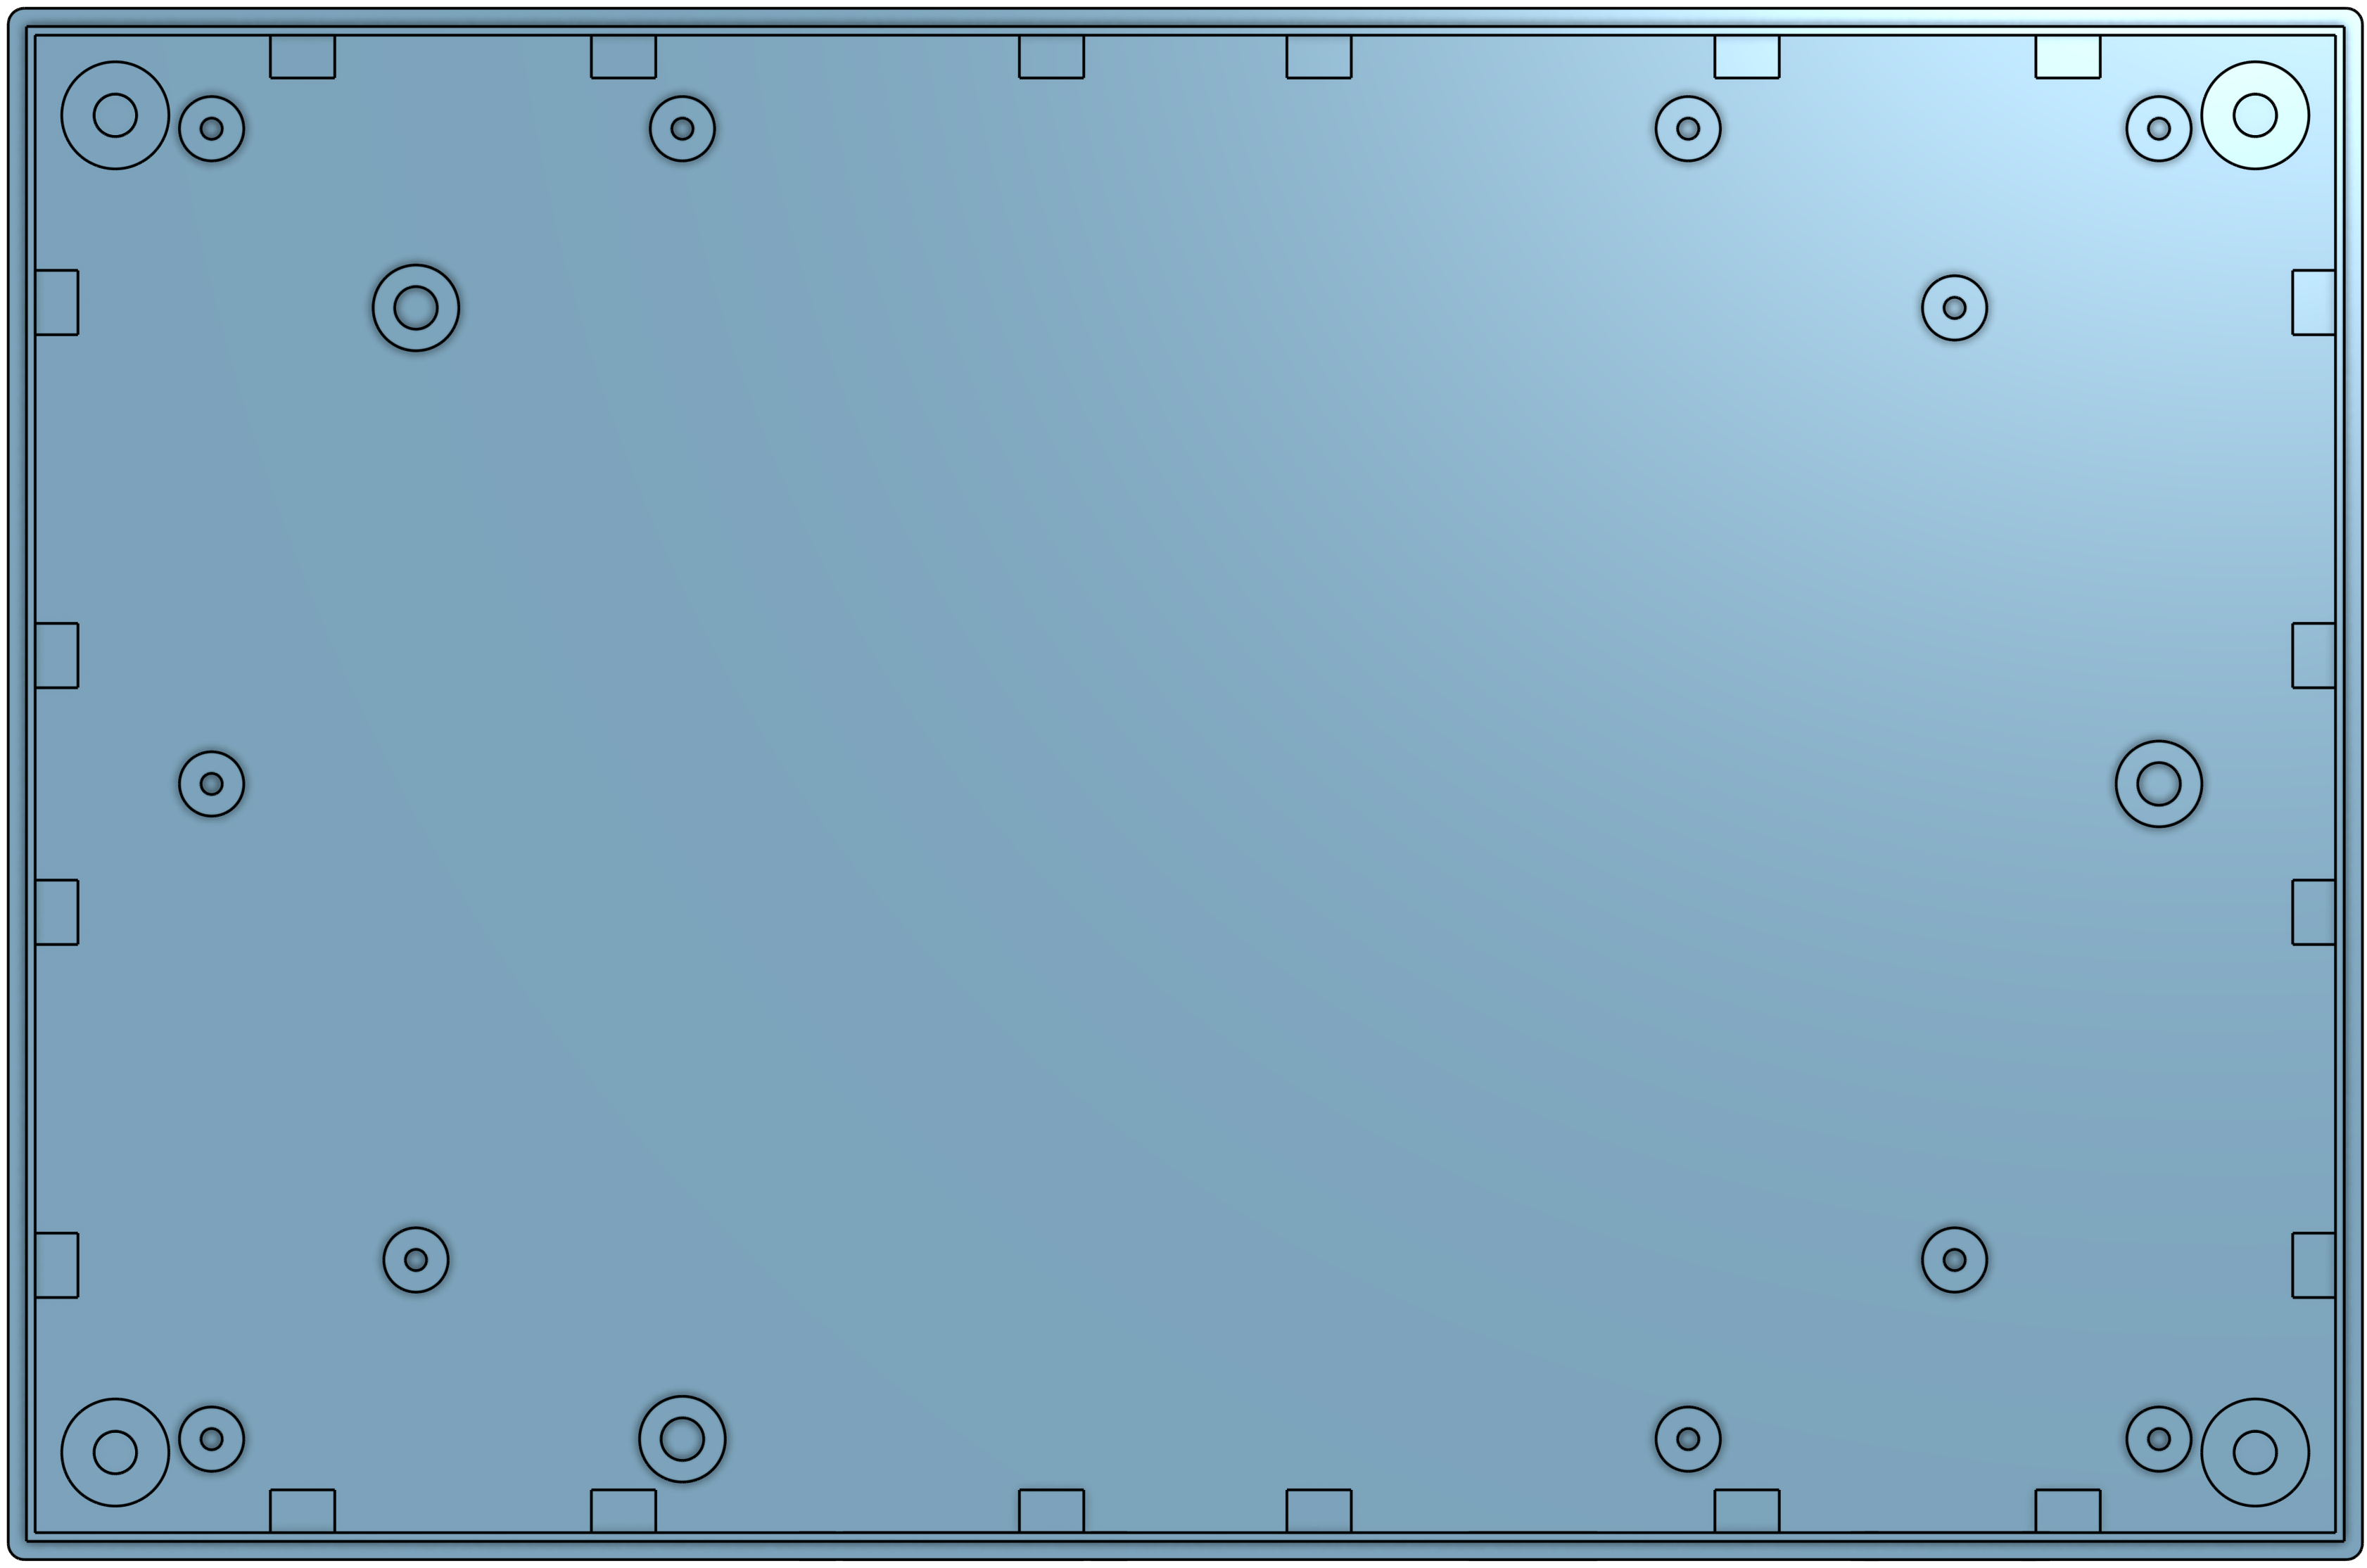
\includegraphics[width=0.5\textwidth]{04-caja/cajabaseplanta.png}
    }
    \caption{(a) Vista general de la base de la caja. (b) Vista de planta de la base de la caja}
    \label{fig:cajabase} 
\end{figure} 


\begin{figure}[hbtp]
    \centering
    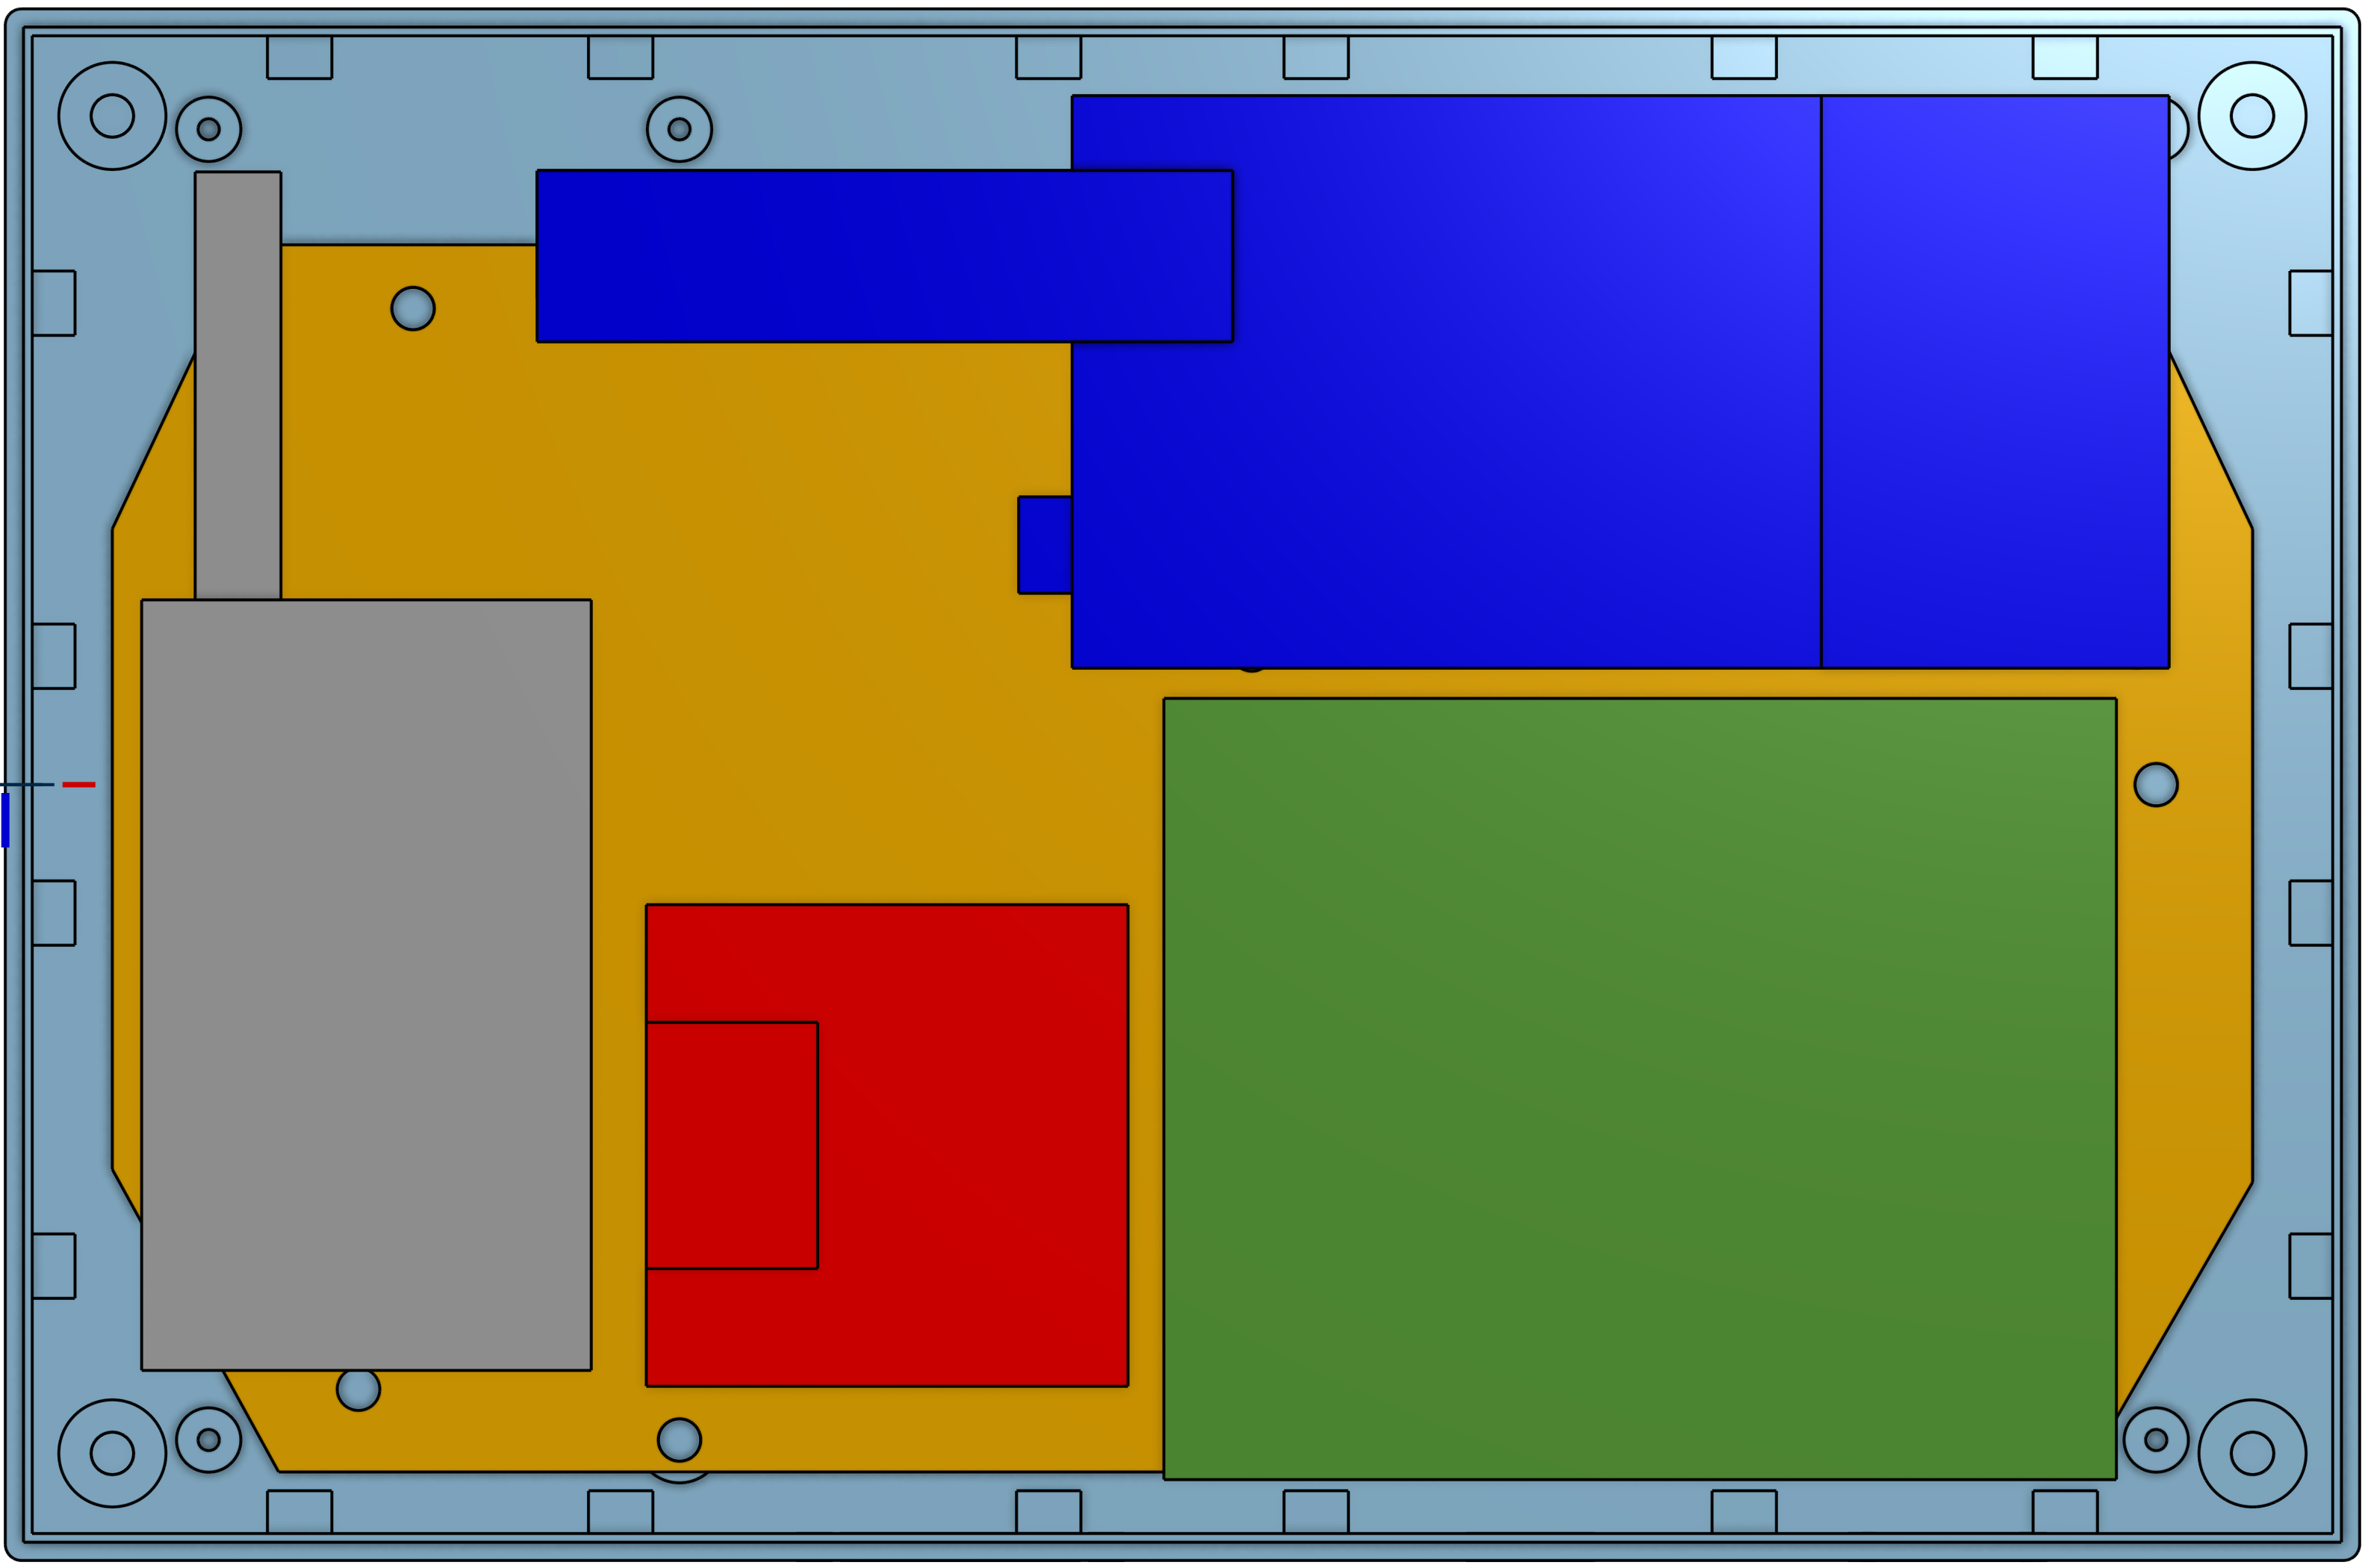
\includegraphics[width=0.5\textwidth]{04-caja/ensamblajebase.png}
    \caption{Ensamblaje de la base con el soporte. Descripción por colores: a) Gris: Fuente. 
    b) Rojo: L298N. c) Azul: Arduino. d) Verde: placa de conexiones. e) Amarillo: Soporte tapa}
    \label{fig:ensamblajebase}
    \end{figure}


\section{Tapa}

La tapa debe ser el soporte para la interfaz humano-máquina y, por ello, sostener todos sus 
dispositivos. Por lo general, todos los dispositivos que van en la tapa son de tamaño reducido,
a excepción de la seta de emergencia, por lo que no hay problemas con su distribución. La seta
de emergencia se ubicará en la esquina superior izquierda, situándose justo encima de la placa
de conexiones del fondo, ya que ésta es la de menor altura. En la figura \ref{fig:cajatapa} se 
muestra la tapa tanto en la planta como en una vista general.

\begin{figure}[h]% 
    \centering 
    \subfloat[][]{% 
        \label{fig:cajatapavista}% 
        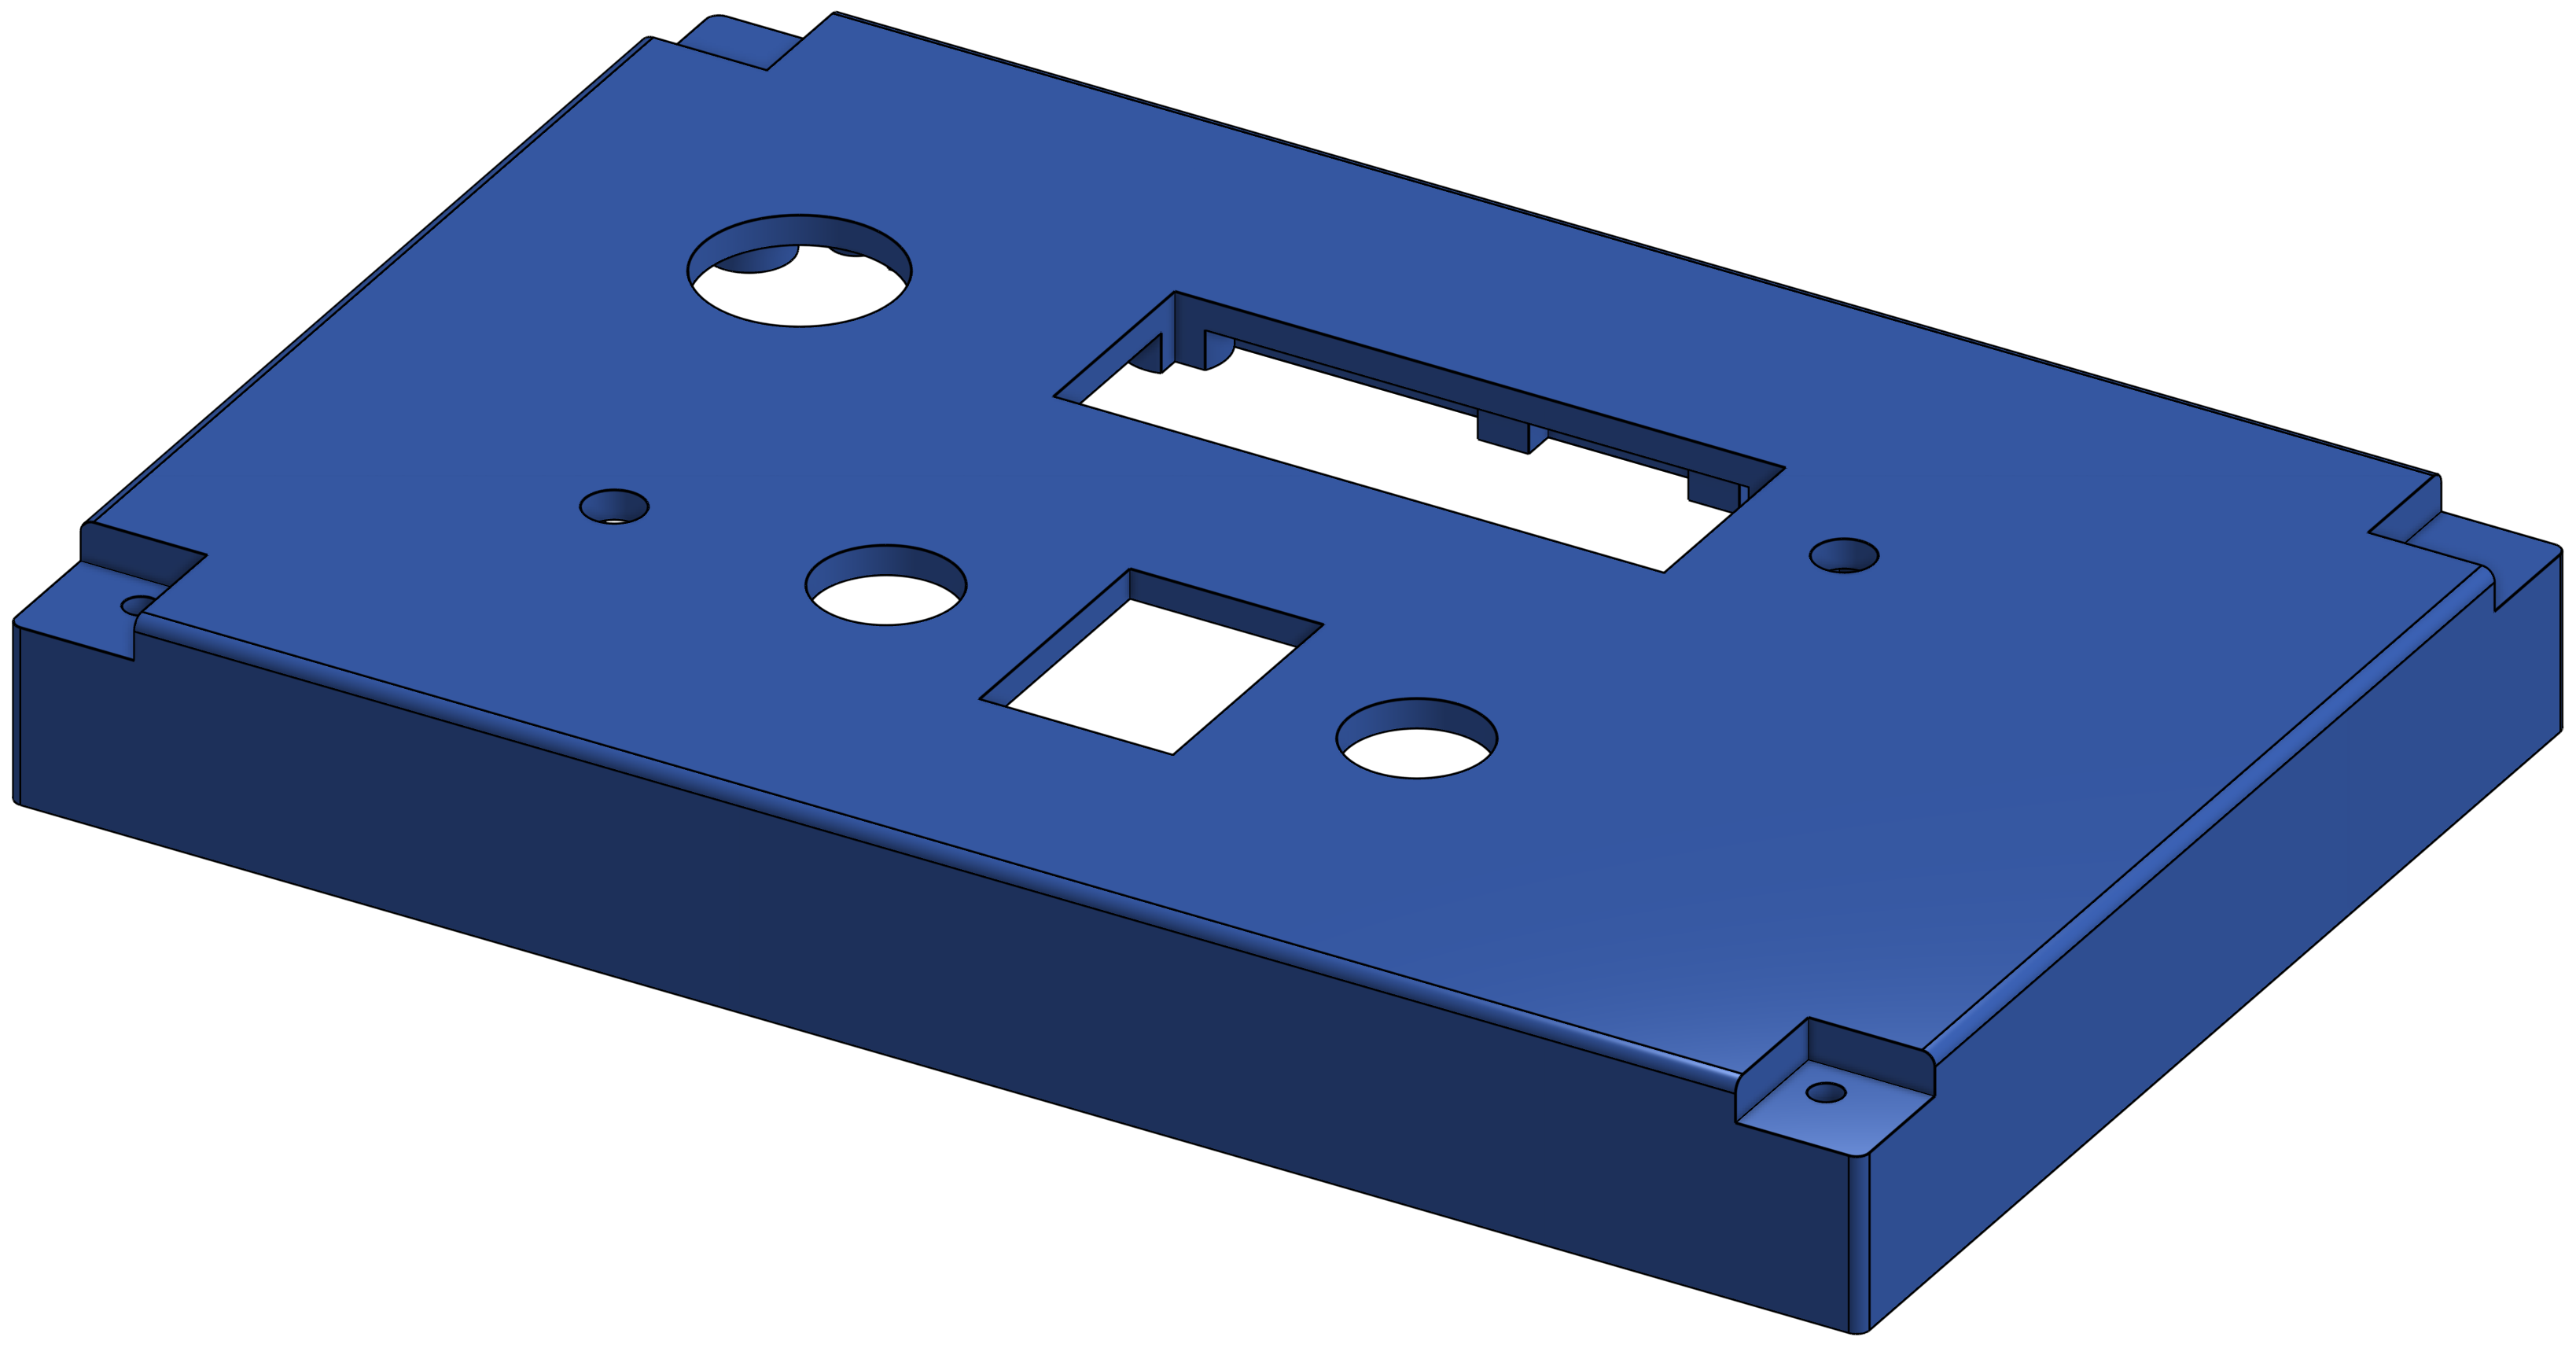
\includegraphics[width=0.5\textwidth]{04-caja/cajatapa.png}
    }% 
    \hspace{10pt}% 
    \subfloat[][]{% 
        \label{fig:cajatapaplanta}% 
        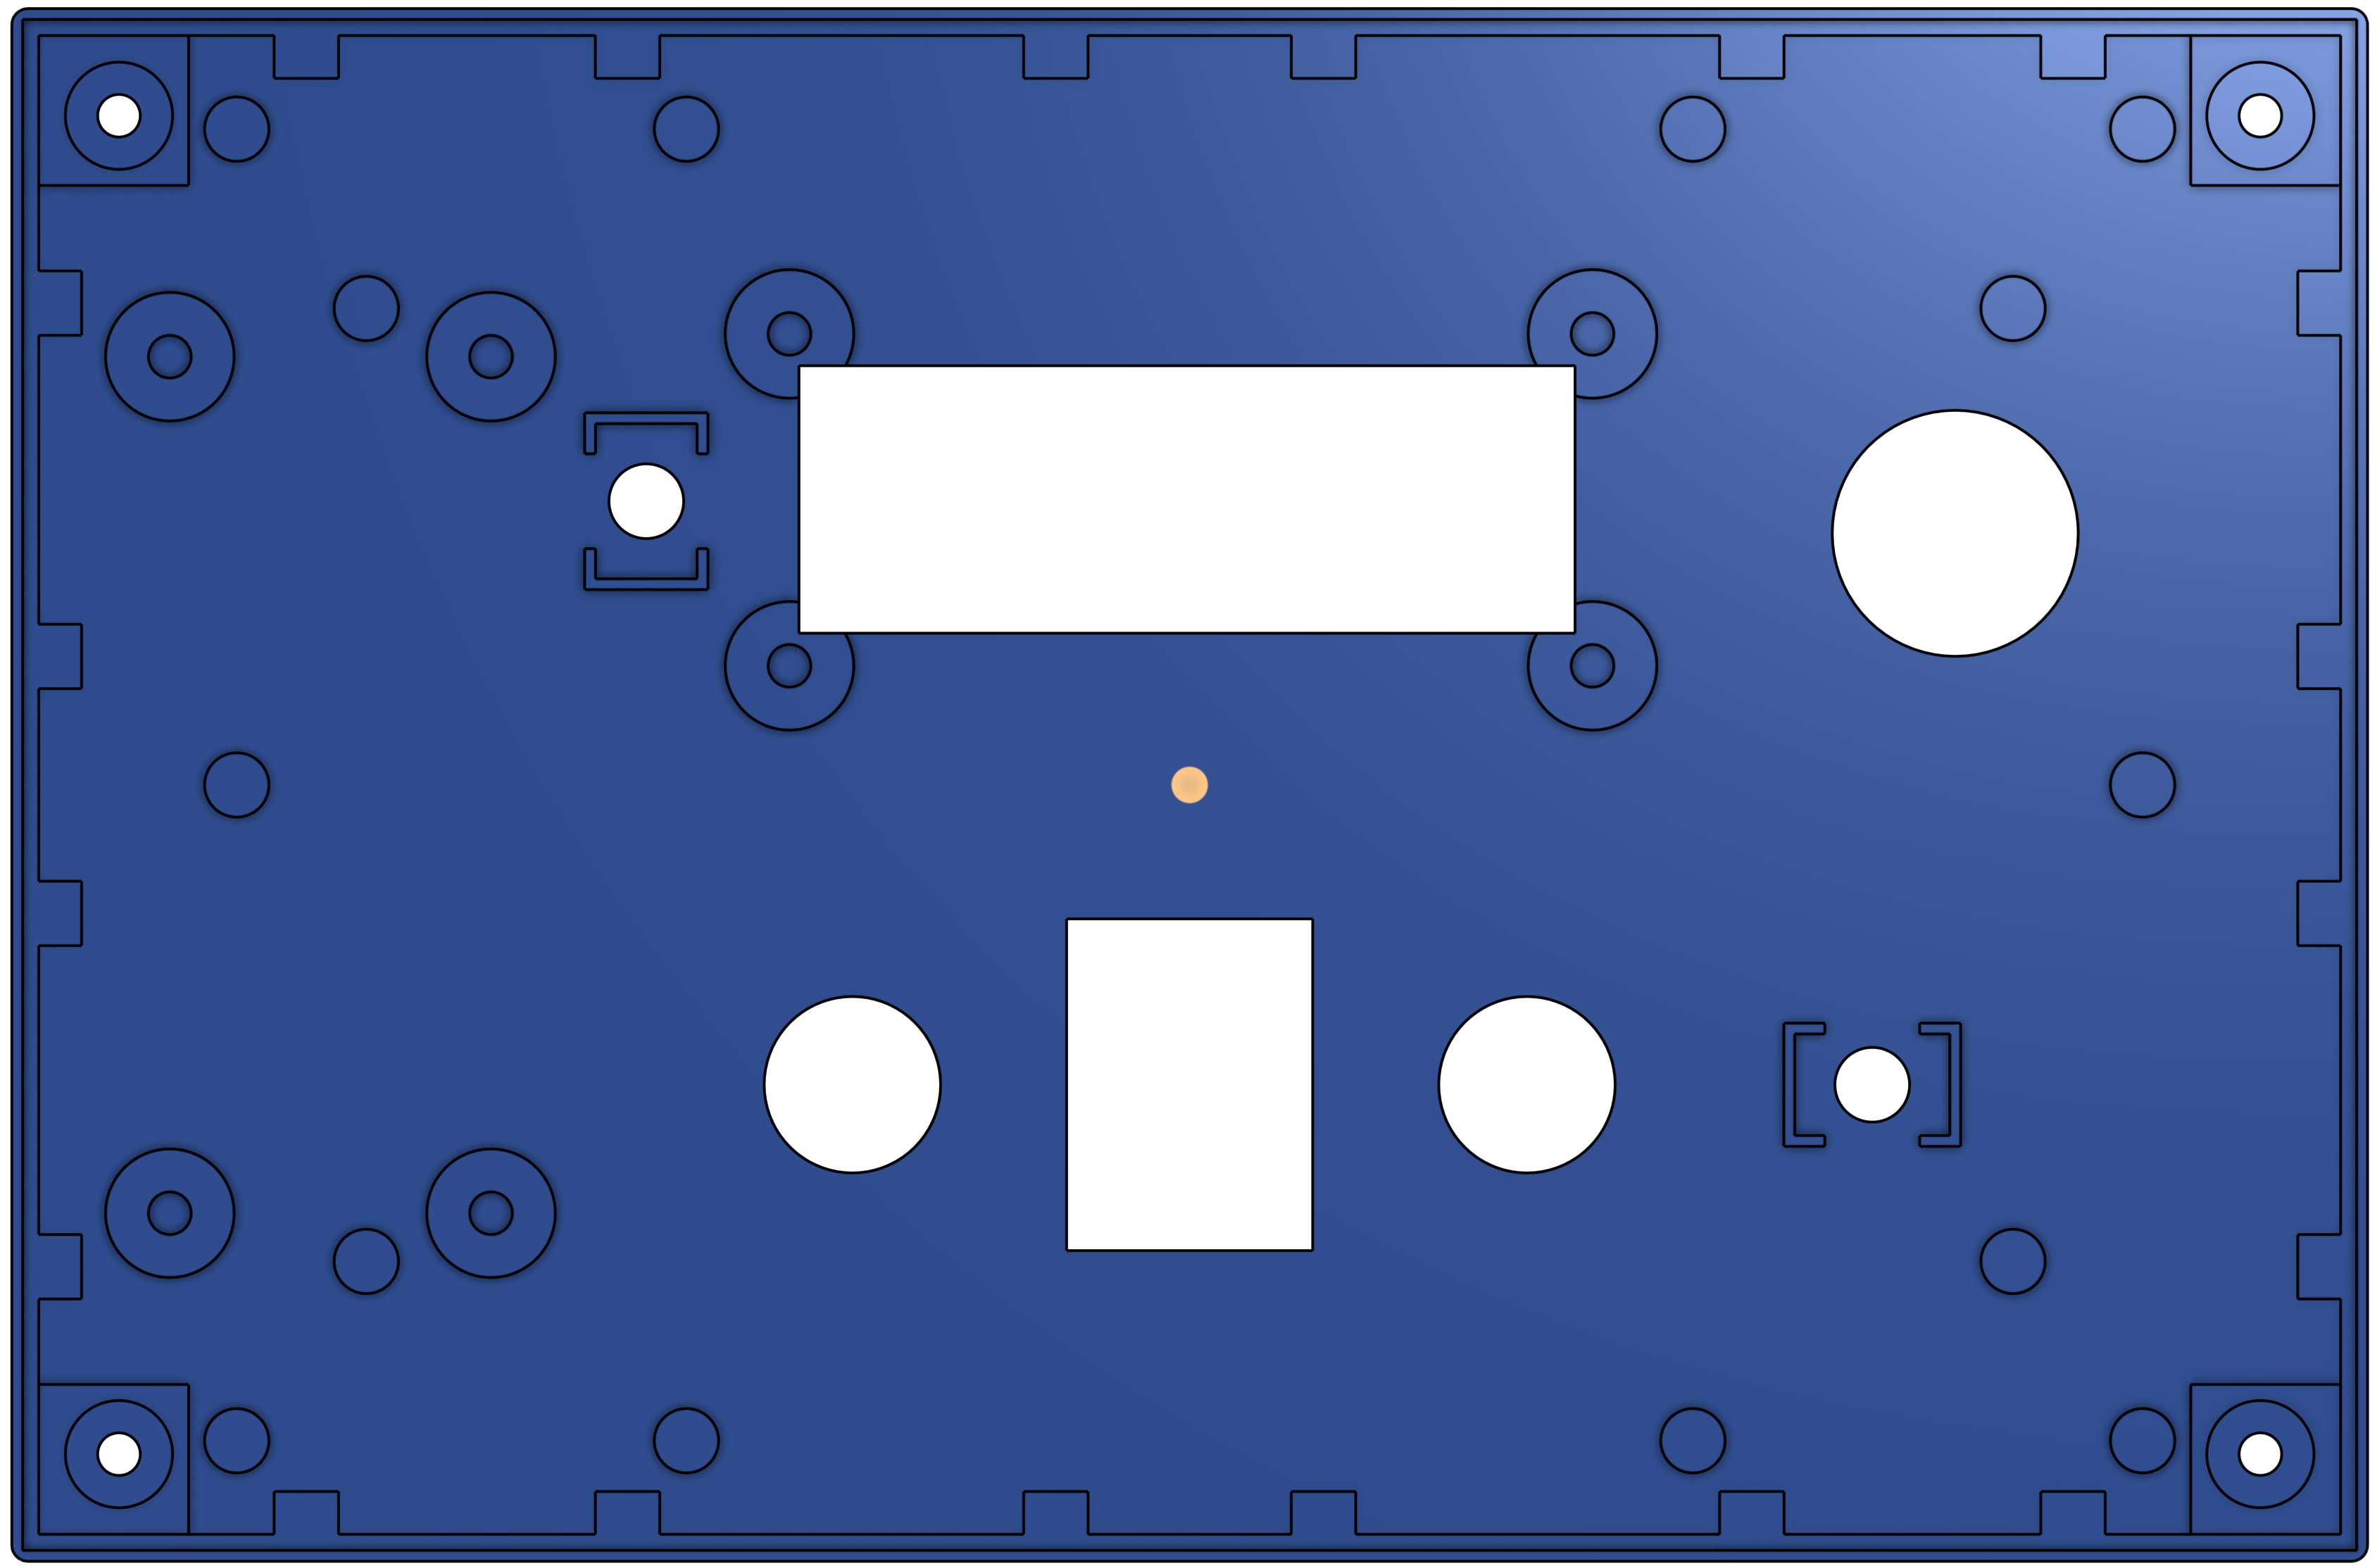
\includegraphics[width=0.5\textwidth]{04-caja/cajatapafondo.png}
    }
    \caption{a) Vista general de la tapa de la caja. b) Vista inferior de la tapa de la caja}
    \label{fig:cajatapa} 
\end{figure} 

Además, se muestra en la figura \ref{fig:cajatapaensamblaje} se muestra la distribución de los 
dispositivos. Ésta distribución permite cumplir con la planificación inicial que se observó en 
la figura \ref{fig:interfazhmi} y facilitar la conexión entre las placas electrónicas al colocar
la línea de interconexión de forma paralela.

\begin{figure}[h]%  
    \centering 
        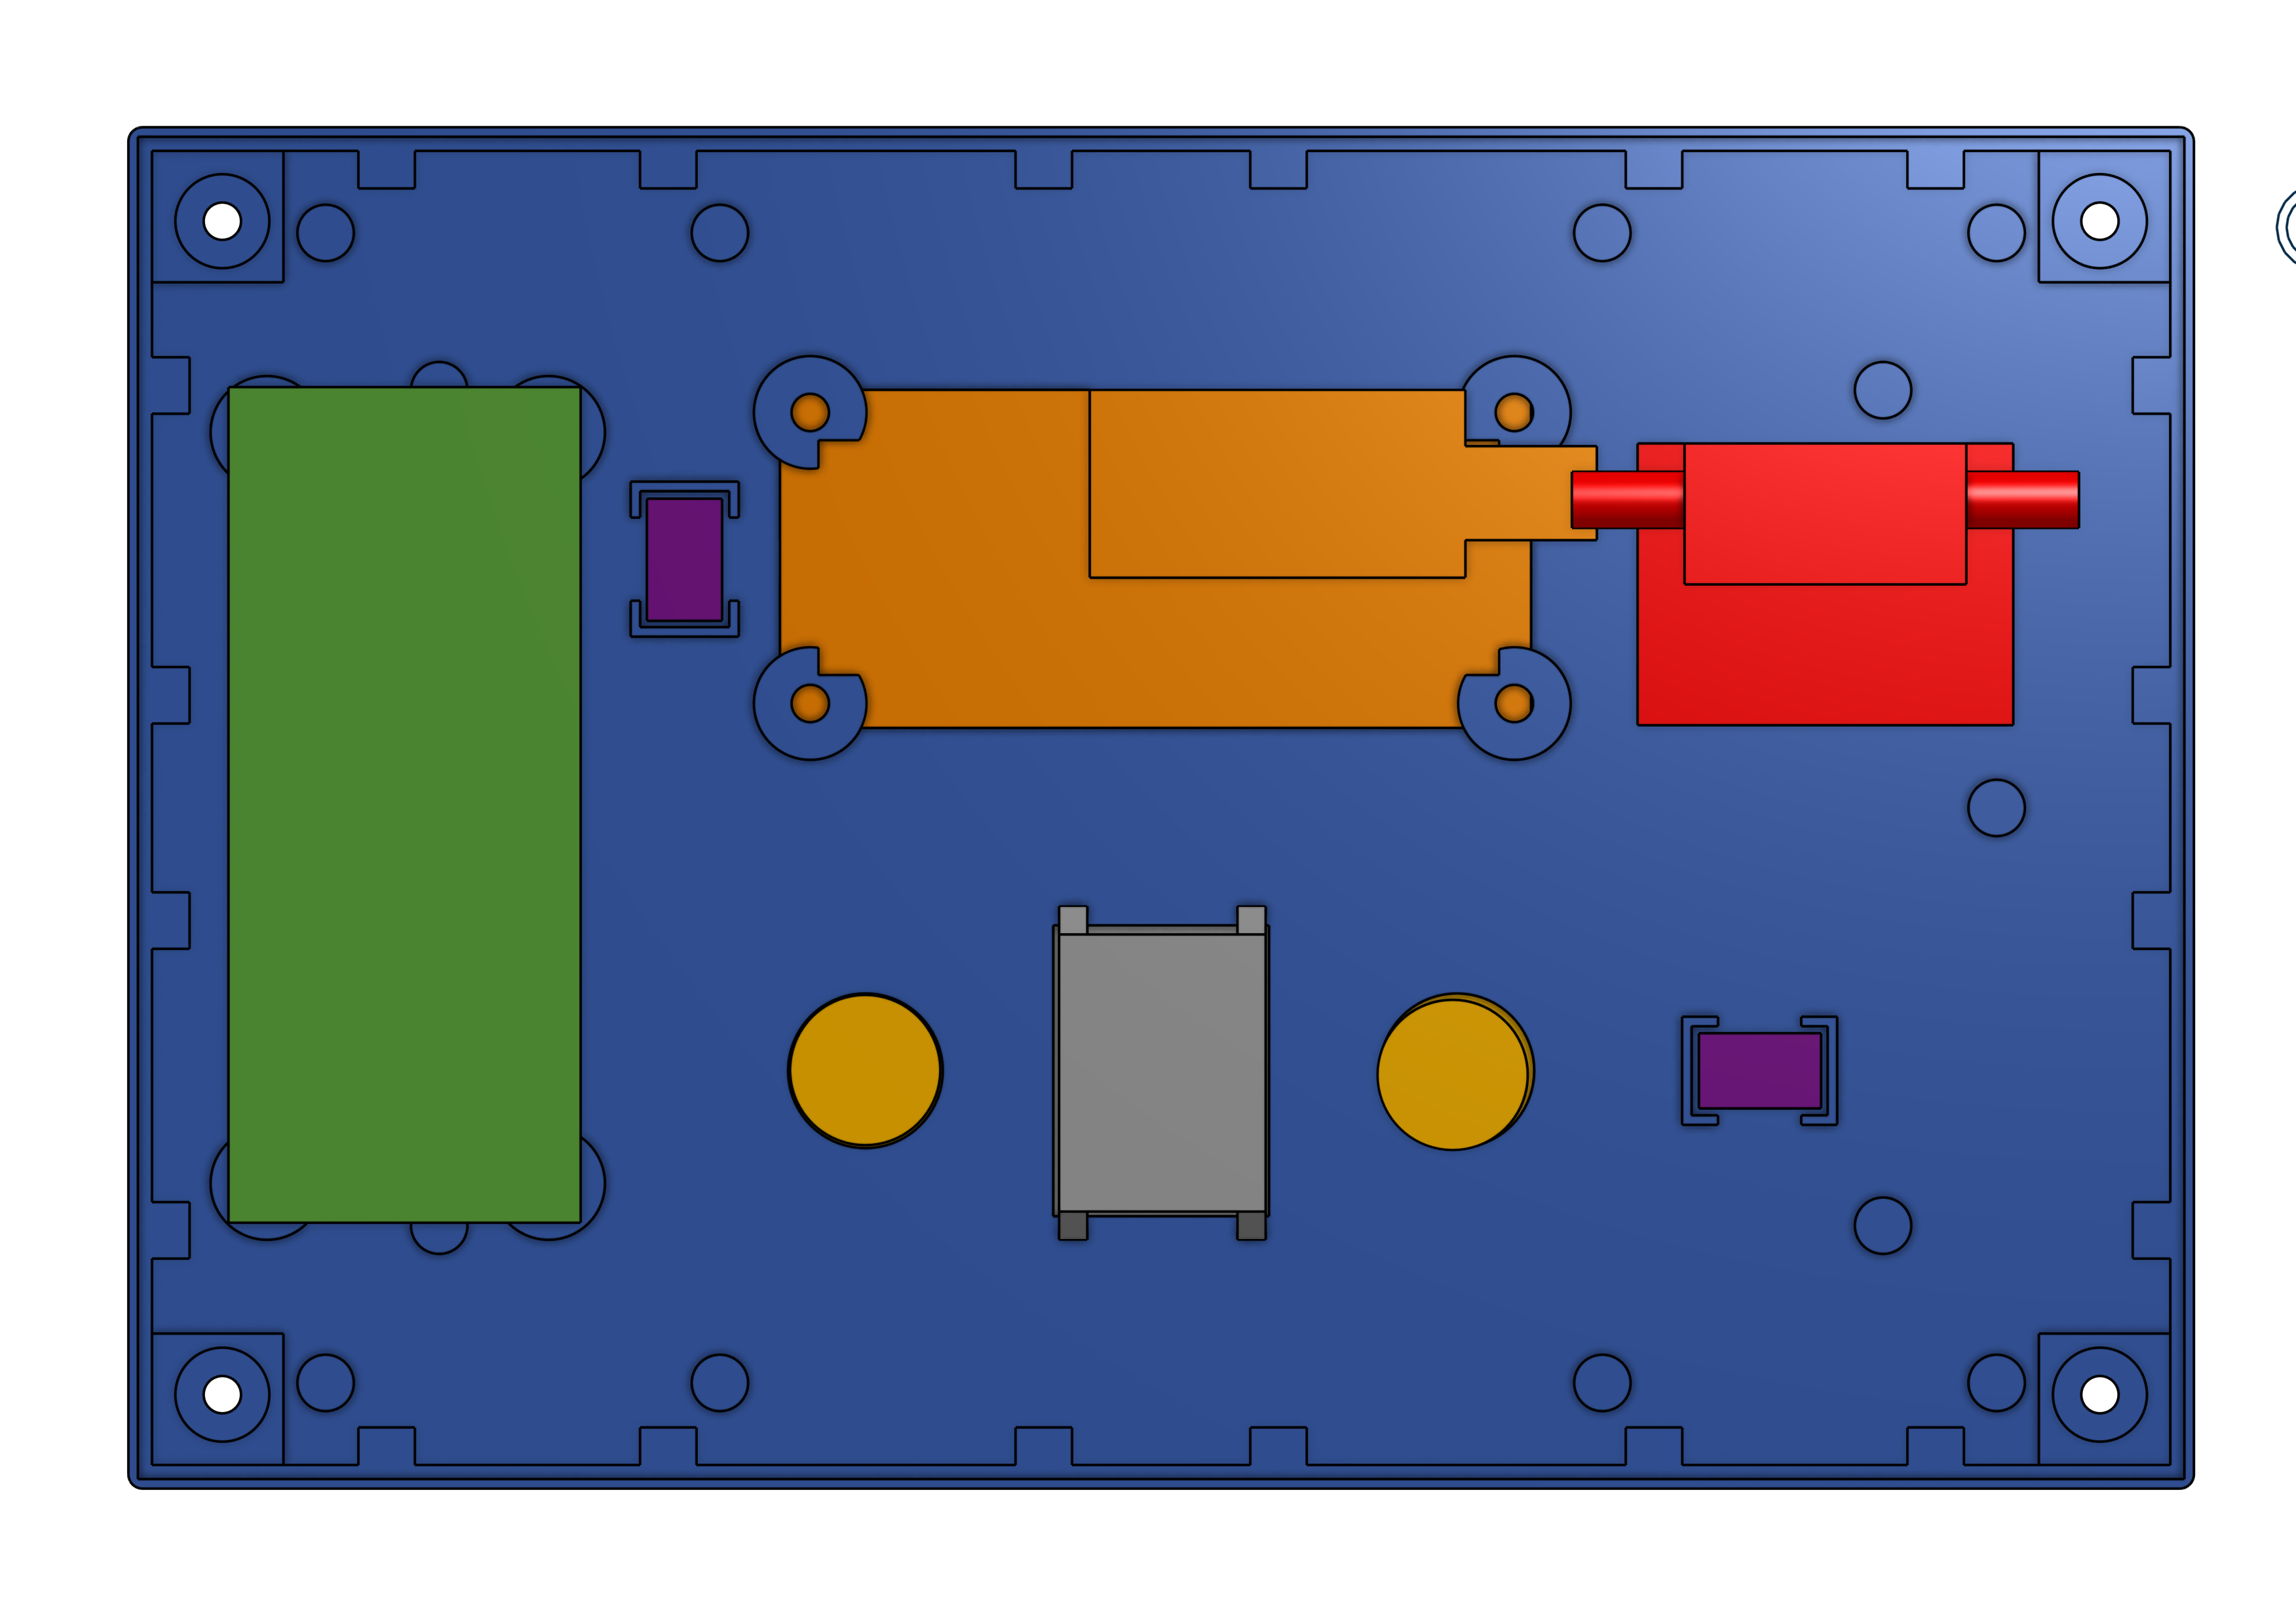
\includegraphics[width=0.5\textwidth]{04-caja/ensamblajetapainferior.png}
    \caption{Vista inferior de la tapa ensamblada. Descripción por colores: a) Verde: placa de 
    conexiones. b) Naranja: LCD c) Rojo: Seta de emergencia. d) Gris: Flechas de selección.
    e) Amarillo: Botones intro y escape. f) Morado: Selectores de modo}
    \label{fig:cajatapaensamblaje} 
\end{figure}